% !TeX spellcheck = en_US
% !TeX root = ./0_article.tex

\section{Logic path under BBI}
For the purpose of analyzing the effects og BBI on actual logic, this section is dedicated in modeling and simulating a more complex logic path, integrating one or more sequential elements.
This implies the use of a clock, governing these elements.
The considered logic path is constituted of inverters, a buffer, and a D Flip-Flop (DFF).
The detailed electrical schematics of each component are described in Fig. \ref{ivxbufmos}, and \ref{dffmos}.

% !TeX spellcheck = en_US
% !TeX root = ./0_article.tex

\begin{figure}[h]
	\label{ivxbufmos}
	\centering
	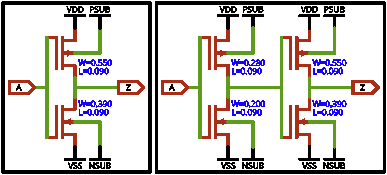
\includegraphics[width=0.5\textwidth]{./figures/IVX_BUFF_X4_3.pdf}
	\caption{IVX MOS SCH \textcolor{red}{A-T-ON LE DROIT DE METTRE CE SCHÉMA ?}}
\end{figure}

% !TeX spellcheck = en_US
% !TeX root = ./0_article.tex

\begin{figure}[h]
	\label{dffmos}
	\center
	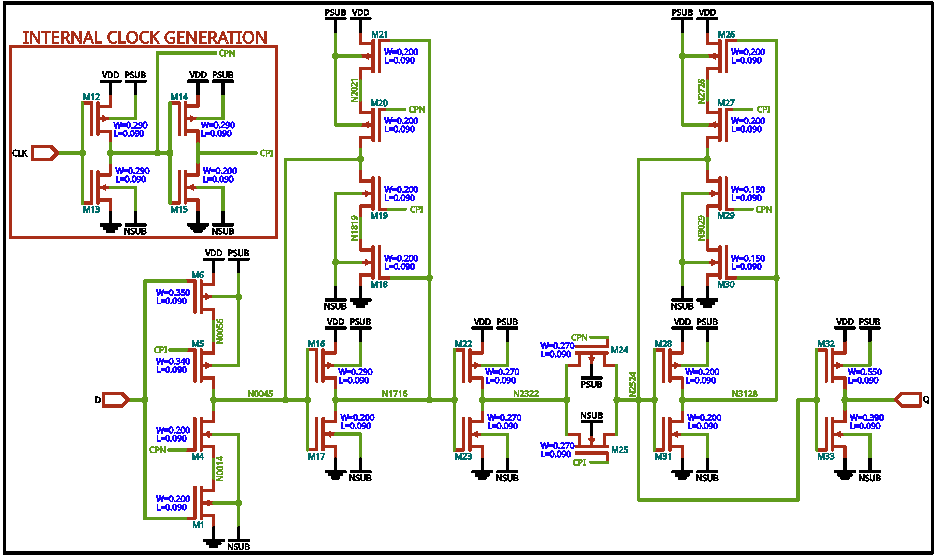
\includegraphics[width=0.5\textwidth]{./figures/CORE65GPSVT_HS65_GS_DFPQX4.pdf}
	\caption{DFF MOS SCH \textcolor{red}{A-T-ON LE DROIT DE METTRE CE SCHÉMA ?}}
\end{figure}


The study is conducted in two scenarios:
\begin{itemize}
	\item When the logic path is static;
	\item When the logic path is dynamic.
\end{itemize}

In this section, we are lingering on analyzing the effects of BBI on more complex logic paths.
The study is conducted for both a static logic path and a dynamic logic path.
The considered logic paths are constituted of inverters, buffers and a D-Flip-Flop (DFF).
The inverters model an arbitrary combinatorial logic path tackling the input of a DFF, used to sample the logic path output.
The DFF clock is buffered to achieve an isolation from the ideal voltage source.
Then, the DFF output is injected into a final 4-IVX chain, loaded with a 5 pF capacitor.
The resulting schematic is described in Fig. \ref{dffChain}.

% !TeX spellcheck = en_US
% !TeX root = ./0_article.tex

\begin{figure}[h]
	\label{dffChain}
	\centering
	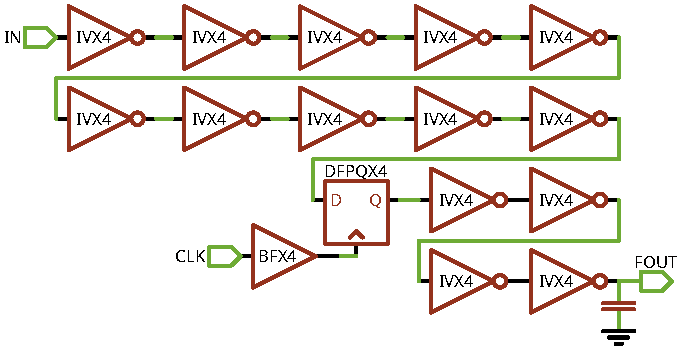
\includegraphics[width=0.5\textwidth]{./figures/dff_ivx_chain_2.pdf}
	\caption{DFFCHAIN}
\end{figure}

